%Este trabalho está licenciado sob a Licença Atribuição-CompartilhaIgual 4.0 Internacional Creative Commons. Para visualizar uma cópia desta licença, visite http://creativecommons.org/licenses/by-sa/4.0/deed.pt_BR ou mande uma carta para Creative Commons, PO Box 1866, Mountain View, CA 94042, USA.

\chapter{Método de elementos finitos em 2D}\label{cap_mef2d}
\thispagestyle{fancy}

\section{Malha e espaço}\label{cap_mef2d_sec_malha}

\subsection{Malha}

Seja $\Omega\subset \mathbb{R}^2$ um domínio limitado com fronteira $\p\Omega$ suave e poligonal. Uma malha (ou triangularização) $\mathcal{K}$ de $\Omega$ é um conjunto de $\{K\}$ células (ou elementos) $K$, tal que $\Omega = \cup_{K\in\mathcal{K}}K$ e tal que a interseção de duas células é ou um lado, um canto ou vazio.

Classicamente as células $K$ são escolhidas como triângulos. O tamanho do lado de maior comprimento do triangulo $K$ define o chamado \emph{tamanho local da malha} $h_K$. O tamanho global da malha é definida por $h = \max_{K\in\mathcal{K}} h_K$.

Uma malha é dita \emph{regular} quando existe uma constante $c_0 > 0$ tal que $c_K > c_0$ para todo $K\in\mathcal{K}$, sendo $c_K := h_K/d_k$ e $d_K$ o diâmetro do circulo inscrito em $K$. Esta condição significa que os triângulo $K$ da malha não podem ter ângulos muito grandes nem muito pequenos. Ao longo do texto, a menos que especificado o contrário, assumiremos trabalhar com malhas regulares.

\subsection{Espaço dos polinômios lineares por partes}

Seja $K$ um triângulo e seja $P_1(K)$ o espaço das funções lineares em $K$, i.e.
\begin{equation}
  P_1(K) = \{v;~v=c_0+c_1x_1+c_2x+2,~(x_1,x_2)\in K,~c_0,c_1,c_2\in\mathbb{R}\}.
\end{equation}

Observemos que toda função $v\in P_1(K)$ é unicamente determinada por seus valores nodais $\alpha_i = v(N_i)$, $i=0, 1, 2$, onde $N_i = (x_1^{(i)}, x_2^{(i)})$ é o $i$-ésimo nodo (vértice) do triângulo $K$. Isto segue do fato de que
\begin{equation}
  \begin{bmatrix}
    1 & x_1^{(1)} & x_2^{(1)}\\
    1 & x_1^{(2)} & x_2^{(2)}\\
    1 & x_1^{(3)} & x_2^{(2)}
  \end{bmatrix}
  \begin{bmatrix}
    c_0\\
    c_1\\
    c_2
  \end{bmatrix} = 
  \begin{bmatrix}
    \alpha_1\\
    \alpha_2\\
    \alpha_3
  \end{bmatrix}
\end{equation}
Computando o valor absoluto do determinante da matriz de coeficientes, obtemos $2|K|$, onde $|K|$ denota a área de $K$, a qual é não nula.

Afim de usarmos os valores nodais como graus de liberdade (incógnitas), nós introduzimos a seguinte base nodal $\{\lambda_1, \lambda_2, \lambda_3\}$ com
\begin{equation}
  \lambda_j(N_i) = \left\{
    \begin{array}{ll}
      1 &, i=j,\\
      0 &, i\neq j
    \end{array}
\right.,~i,j=0,1,2.
\end{equation}
Com esta base, toda função $v\in P_1(K)$ pode ser escrita como
\begin{equation}
  v = \alpha_1\lambda_1 + \alpha_2\lambda_2 + \alpha_3\lambda_3,
\end{equation}
onde $\alpha_i = v(N_i)$.

\subsection{Espaço contínuo dos polinômios lineares por partes}

O espaço contínuo dos polinômios lineares por partes na malha $\mathcal{K}$ é definido por
\begin{equation}
  V_h = \{v;~v\in C^0(\Omega),~v|_K\in P_1(K),~\forall K\in\mathcal{K}\}.
\end{equation}

Observemos que toda função $v\in V_h$ é unicamente determinada por seus valores nodais $\{v(N_j)\}_{j=1}^{n_p}$, onde $n_p$ é número de nodos da malha $\mathcal{K}$. De fato, os valores nodais determinam uma única função em $P_1(K)$ para cada $K\in\mathcal{K}$ e, portanto, uma função em $V_h$ é unicamente determinada por seus valores nos nodos. Agora, consideremos dois triângulos $K_1$ e $K_2$ compartilhando um lado $E = K_1\cap K_2$. Sejam $v_1$ e $v_2$ os dois únicos polinômios em $v_1\in P_1(K_1)$ e $v_2\in P_2(K_2)$, respectivamente determinados pelos valores nodais em $K_1$ e $K_2$. Como $v_1$ e $v_2$ também são polinômios lineares em $E$ e seus valores coincidem nos nodos de $E$, temos $v_1 = v_2$. Portanto, concluímos que toda função $v\in V_h$ é unicamente determinada por seus valores nodais.

Afim de termos os valores nodais como graus de liberdade (incógnitas), definimos a base nodas $\{\phi_j\}_{j=1}^{n_p}\subset V_h$ tal que
\begin{equation}
  \varphi_j(N_i) = \left\{
    \begin{array}{ll}
      1 &, i=j\\
      0 &, i\neq j
    \end{array}
\right.,~i,j=0, 1, \dotsc, n_p-1.
\end{equation}
Notemos que cada função base $\phi_j$ é contínua, linear por partes e com suporte somente em um pequeno conjunto de triângulos que compartilham o nodo $N_j$. Além disso, todo a função $v\in V_h$ pode, então, ser escrita como
\begin{equation}
  v = \sum_{i=0}^{n_p-1}\alpha_i\varphi_i,
\end{equation}
onde $\alpha_i = v(N_i)$, $i=0, 1, \ldots, n_p$, são os valores nodais de $v$.

\begin{ex}\label{ex:malha}
  A Figura \ref{fig:ex_malha} mostra o esboço de uma malha triangular no domínio $D = [0, 1]\times [0, 1]$.

  \begin{figure}[h!]
    \centering
    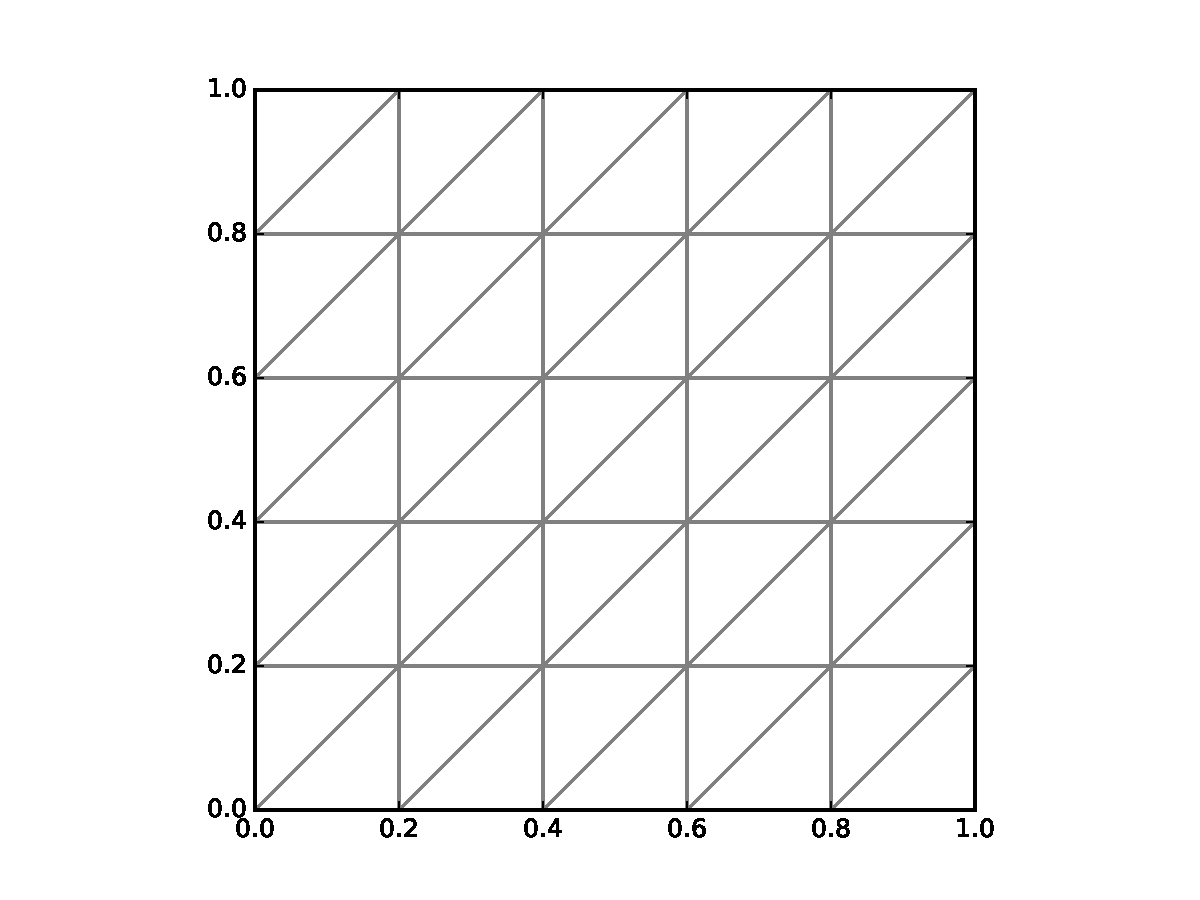
\includegraphics[width=0.7\textwidth]{./cap_mef2d/dados/ex_malha/fig_ex_malha}
    \caption{Esboço de uma malha triangular no domínio $D = [0, 1]\times [0, 1]$.}
    \label{fig:ex_malha}
  \end{figure}

\ifispython
Com o \fenics, podemos gerar esta malha com o seguinte \href{https://github.com/phkonzen/notas/blob/master/src/MetodoElementosFinitos/cap_mef2d/dados/ex_malha/ex_malha.py}{código}:
\verbatiminput{./cap_mef2d/dados/ex_malha/ex_malha.py}
\fi
\end{ex}

\section{Interpolação e projeção}\label{cap_mef2d_sec_interp}

\subsection{Interpolação}

Dada uma função contínua $f$ em um triângulo $K$ com nodos $N_i$, $i=0, 1, 2$, sua interpolação linear $\phi f \in P_1(K)$ é definida por
\begin{equation}
  \pi f = \sum_{i=0}^3 f(N_i)\varphi_i.
\end{equation}
Logo, temos $\pi f(N_i) = f(N_i)$ para todo $i=0, 1, 2$.

Afim de determinarmos estimativas para o erro de interpolação, precisamos da chamada derivada total de primeira ordem
\begin{equation}
  Df = \left(\left|\frac{\p f}{\p x_1}\right|^2 + \left|\frac{\p f}{\p x_2}\right|^2\right)^{1/2},
\end{equation}
e da derivada total de segunda ordem
\begin{equation}
  D^2f = \left(\left|\frac{\p^2 f}{\p x_1^2}\right|^2 + \left|\frac{\p^2 f}{\p x_1\p x_2}\right|^2 + \left|\frac{\p^2 f}{\p x_2^2}\right|^2\right)^{1/2}.
\end{equation}

\begin{prop}\normalfont{(Erro da interpolação no espaço linear)}\label{prop:interpl}
  A interpolação $\pi f$ satisfaz as seguintes estimativas
  \begin{align}
    \|f - \pi f\|_{L^2(K)} &\leq Ch_K^2\|D^2f\|_{L^2(K)},\label{eq:interpl_0}\\
    \|D(f - \pi f)\|_{L^2(K)} &\leq Ch_K\|D^2 f\|_{L^2(K)}.\label{eq:interpl_1}
  \end{align}
\end{prop}
\begin{dem}
  Veja \cite[Capítulo 4]{Brenner2008a}.
\end{dem}

\begin{obs}
  A constante $C$ dependo do inverso de $\sen(\theta_K)$ onde $\theta_K$ é o menor angulo de $K$. Desta forma, para um triângulo com $\theta_K$ muito pequeno, as estimativas \eqref{eq:interpl_0} e \eqref{eq:interpl_1} perdem sentido. Este fato indica a necessidade de se trabalhar com malhas regulares.
\end{obs}

A interpolação no espaço $V_h$ de uma dada função $f$ no domínio $\Omega$ é denotada também por $\pi f\in V_h$ e definida por
\begin{equation}
  \pi f = \sum_{i=0}^{n_p-1} f(N_i)\varphi_i.
\end{equation}

\begin{prop}\normalfont{(Erro da interpolação no espaço contínuo linear por partes)}\label{prop:interpc}
  O interpolador $\pi f\in V_h$ satisfaz as seguintes estimativas
  \begin{align}
    \|f - \pi f\|_{L^2(\Omega)}^2 &\leq C\sum_{K\in\mathcal{K}} h_K^4\|D^2 f\|_{L^2(K)}^2,\label{eq:interpc_0}\\
    \|D(f - \pi f)\|_{L^2(\Omega)}^2 &\leq C\sum_{K\in\mathcal{K}} h_K^2\|D^2 f\|_{L^2(K)}^2,\label{eq:interpc_1}.
  \end{align}
\end{prop}
\begin{dem}
  Demonstração análoga a Proposição \ref{prop:interp_linpartes}.
\end{dem}

\ifispython
\begin{ex}\label{ex:interp}
Consideremos a função $f(x_0,x_1) = \sen(\pi x_0)\cos(\pi x_1)$ definida no domínio $D = [0, 1]\times [0, 1]$. O seguinte \href{https://github.com/phkonzen/notas/blob/master/src/MetodoElementosFinitos/cap_mef2d/dados/ex_interp/ex_interp.py}{código} computa a interpolação de $f$ no espaço $V_h$ sobre uma malha triangular uniforme.

\verbatiminput{./cap_mef2d/dados/ex_interp/ex_interp.py}
\end{ex}
\fi

\subsection{Projeção $L^2$}

A projeto $L^2$ no espaço $V_h$ de uma dada uma função $f\in L^2(\Omega)$  é denotada por $P_hf\in V_h$ e definida por
\begin{equation}
  \int_\Omega (f-P_hf)v\,dx = 0,~\forall v\in V_h.
\end{equation}

Analogamente a projeção em uma dimensão (veja Subseção \ref{subsec:projecao_1d}), a projeção
\begin{equation}
  P_h f = \sum_{j=0}^{n_p-1} \xi_j\varphi_j,
\end{equation}
onde $\xi_j$ satisfaz o sistema linear
\begin{equation}
  M\pmb{\xi} = \pmb{b},
\end{equation}
onde $M = [m_{i,j}]_{i,j=0}^{n_p-1}$ é a matriz de massa com
\begin{equation}
  m_{i,j} = \int_{\Omega} \varphi_i\varphi_j\,dx
\end{equation}
e $\pmb{b} = (b_1,~b_2,~\dotsc,~b_{n_p-1})$ é o vetor de carga com
\begin{equation}
  b_i = \int_\Omega f\varphi_i\,dx.
\end{equation}

Também, vale o resultado análogo da melhor aproximação (veja \ref{teo:melhor_aprox}), i.e.
\begin{equation}
  \|f-P_hf\|_{L^2(\Omega)} \leq \|f - v\|_{L^2(\Omega)},\quad\forall v\in V_h.
\end{equation}
E, portanto, também temos a estimativa análoga para o erro de projeção (veja \ref{teo:erro_proj_1d})
\begin{equation}
  \|f-P_hf\|_{L^2(\Omega)}^2 \leq C\sum_{K\in\mathcal{K}} h_K^4\|D^2 f\|_{L^2(K)}^2.
\end{equation}
Tomando o tamanho global da malha, temos
\begin{equation}\label{eq:erro_projec_2d}
  \|f-P_hf\|_{L^2(\Omega)} \leq Ch^2\|D^2 f\|_{L^2(K)}.
\end{equation}

\ifispython
\begin{ex}\label{ex:projec}
Consideremos a função $f(x_0,x_1) = \sen(\pi x_0)\cos(\pi x_1)$ definida no domínio $D = [0, 1]\times [0, 1]$. O seguinte \href{https://github.com/phkonzen/notas/blob/master/src/MetodoElementosFinitos/cap_mef2d/dados/ex_projec/ex_projec.py}{código} computa a projeção de $f$ no espaço $V_h$ sobre uma malha triangular uniforme.

\verbatiminput{./cap_mef2d/dados/ex_projec/ex_projec.py}
\end{ex}
\fi

\subsection*{Exercícios}

\begin{exer}
  Verifique computacionalmente a Proposição \ref{prop:interpc} no caso da função $f(x_0,x_1) = \sen(\pi x_0)\cos(\pi x_1)$ interpolada sobre uma malha triangular uniforme sobre o domínio $D = [0, 1]\times [0, 1]$.
\end{exer}

\begin{exer}
  Verifique computacionalmente a estimativa \eqref{eq:erro_projec_2d} no caso da função $f(x_0,x_1) = \sen(\pi x_0)\cos(\pi x_1)$ projetada sobre uma malha triangular uniforme sobre o domínio $D = [0, 1]\times [0, 1]$.
\end{exer}